
\subsection{Comparando Arquitecturas}

Ahora que se conoce el estado actual del sistema, al igual que estado de referencia; lo siguiente a realizar era la comparación de las arquitecturas. El resultado de esta, nos daría la base para poder decidir el qué hacer para adaptar el sistema y el cómo hacerlo.

En la figura \ref{fig:StarDuckBasic}, uno de los servicios intermedios estaba encargado de manejar la base de conocimiento. Este contiene las versiones actualizadas de la arquitectura de referencia, enviada a este desde el cliente de Lexical usado por el usuario; y el estado actual, que Looker está constantemente actualizando, y puede ser consultado por este servicio cada que se requiera. Siendo así, este servicio será el encargado de realizar las comparaciones entre los dos estados.

Ya teniendo definido dónde se realizarán las comparaciones, lo siguiente es definir el como se realizarán estas. Para nuestras necesidades, esto no es tan directo como hacer una comparación usando un igual (\texttt{A == B}) ya que el realizar esto, no nos daría realmente información sobre, qué, internamente, presenta problemas.

Para poder extraer esta información, siendo esta el estado de los componentes específicos que necesitan atendidos, se estableció el uso de métricas definidas con anterioridad. En este caso, las métricas elegidas son el tiempo entre mensajes de los dispositivos y la cantidad de estos en una locación.

El proceso de comparación consta de evaluar cada componente del sistema en función de estas métricas. Se comparan las versiones objetivo y actual para determinar si hay discrepancias significativas que requieran ajustes. Si, por ejemplo, el tiempo entre mensajes de un dispositivo en una ubicación difiere de la versión objetivo, se considera que hay una desviación. Lo mismo ocurre si la cantidad de dispositivos en una locación no coincide con la definición de la arquitectura objetivo.

Lo siguiente a realizar fue definir el proceso de comparación entre los dos estados del sistema. Se optó por abordar esta comparación locación por locación, permitiendo así una evaluación detallada de cada área y extrayendo una estructura que resaltara los puntos problemáticos de la aplicación y las diferencias presentes en cada uno de los lugares. 

Siendo así, primeramente se definió el flujo en el cual se realizará el recorrido de las locaciones. Se parte desde las locaciones raíces, o de primer nivel, y pasando por cada una de las locaciones hijas revisando el estado de cada una de estas. En la figura \ref{fig:BranProcess} se presenta el diagrama de flujo de la forma en la que se realizará el recorrido de las locaciones.

\begin{figure}[H]
    \centering
    \caption{Diagrama de flujo del recorrido de las locaciones}
    \label{fig:BranProcess}
    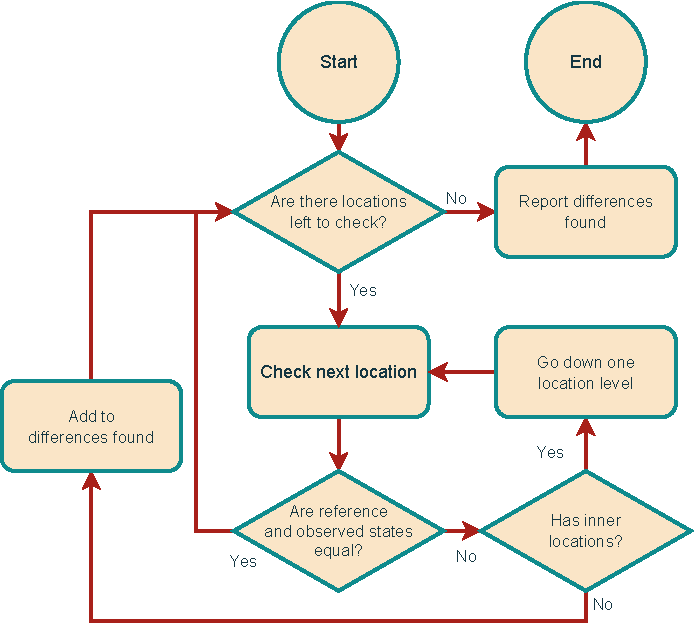
\includegraphics[width=0.8\linewidth]{images/BranProcess.pdf}
\end{figure}

En cada una de las locaciones que se visita, se compara el estado de cada uno de los componentes definidos en la arquitectura de referencia. Esta comparación se basa en revisar tres cosas. Primero, si el componente está presente en la locación; segundo, como fue definido en la sección anterior, si se han estado mandando mensajes dentro del tiempo establecido; y, finalmente, si se está recibiendo el tipo de dato esperado.

Estos puntos de comparación nos permiten establecer si el componente está presente y activo en la locación; al igual que el tipo de| dato registrados sean coherentes con las necesidades de la aplicación. El diagrama de flujo del proceso defino se puede observar en la figura \ref{fig:BranCompare}.

\begin{figure}[H]
    \centering
    \caption{Diagrama de flujo del proceso de comparación de los componentes}
    \label{fig:BranCompare}
    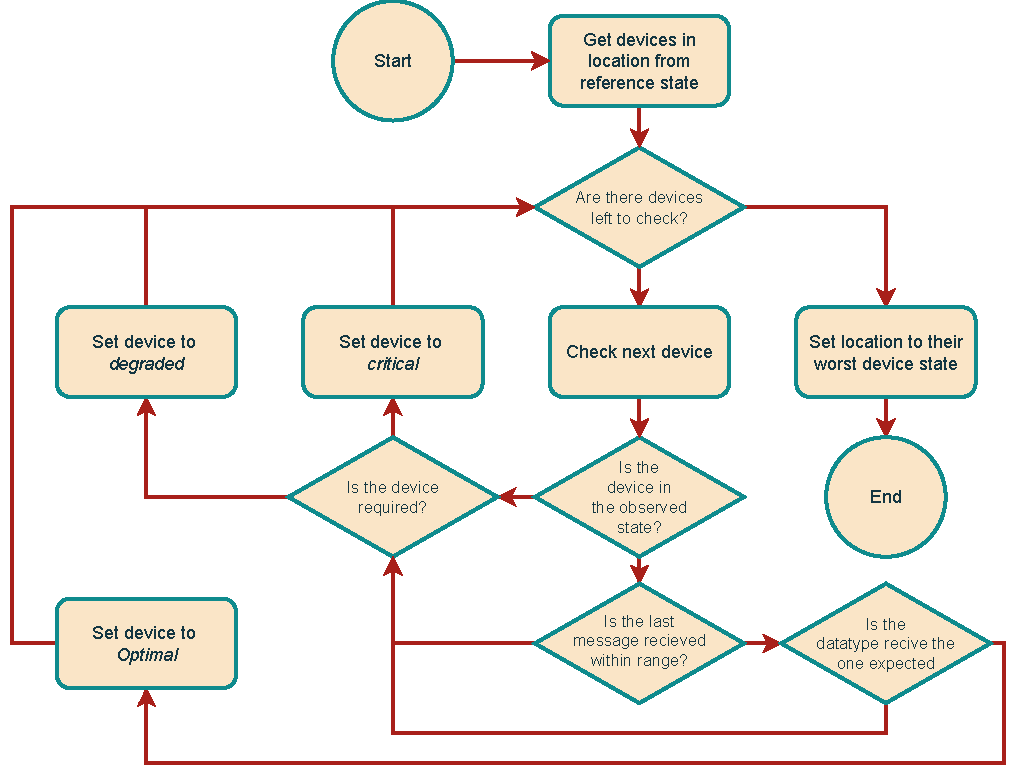
\includegraphics[width=\linewidth]{images/BranCompare.pdf}
\end{figure}

A partir de la información recolectada durante la comparación entre los dos estados, como se puede ver en la figura \ref{fig:BranProcess}, se genera un reporte el cual contiene las locaciones y los dispositivos que presenten problemas. A partir de este, se establecerán las medidas a tomar con el fin de adaptar el sistema hacia un estado óptimo.

